\begin{figure}
    \centering
    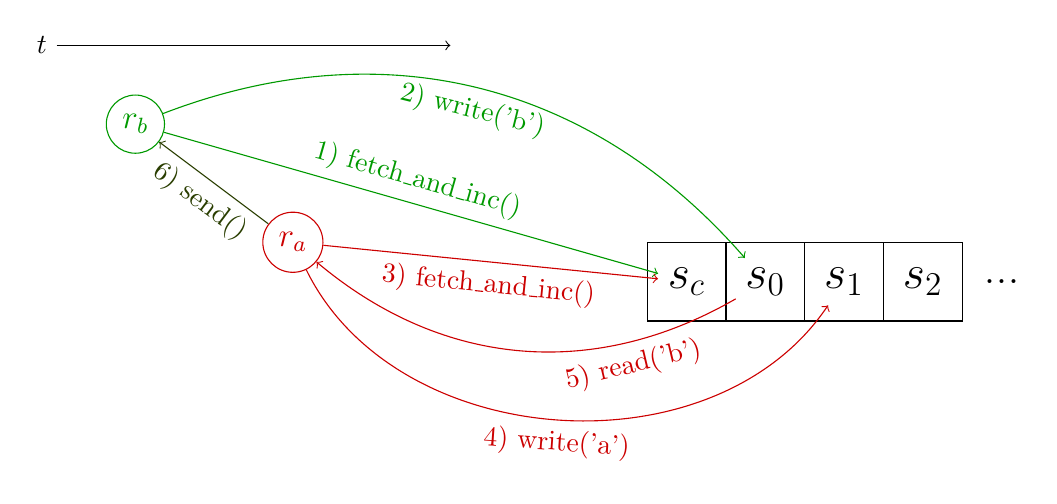
\begin{tikzpicture}[
        nsty/.style={circle,draw,font=\large},
        ssty/.style={font=\LARGE},
        ]
    
        \node (sc) at (1,0) [ssty] {$s_c$};
        \node (s0) at (2,0) [ssty] {$s_0$};
        \node (s1) at (3,0) [ssty] {$s_1$};
        \node (s2) at (4,0) [ssty] {$s_2$};
        \node (scont) at (5,0) [ssty] {...};
        
        \node (ra) at (-4,0.5) [nsty,color=red!80!black] {$r_a$};
        \node (rb) at (-6,2) [nsty,color=green!60!black] {$r_b$};
    
        \draw[->]  (-7,3) node[left] {$t$} --  (-2,3);
    
        \draw (0.5,-0.5) rectangle (1.5,0.5);
        \draw (1.5,-0.5) rectangle (2.5,0.5);
        \draw (2.5,-0.5) rectangle (3.5,0.5);
        \draw (3.5,-0.5) rectangle (4.5,0.5);
    
        \draw[->,color=green!60!black] (rb) -- node[above,sloped,color=green!60!black] {1) fetch\_and\_inc()} (sc);
        \draw[->,color=green!60!black] (rb) to [bend left=35] node[below,sloped,color=green!60!black] {2) write('b')} (s0);
        \draw[->,color=red!80!black] (ra) -- node[below,sloped,color=red!80!black] {3) fetch\_and\_inc()} (sc);
        \draw[->,color=red!80!black] (ra) to [bend right=60] node[below,sloped,color=red!80!black] {4) write('a')} (s1);
        \draw[->,color=red!80!black] (s0) to [bend left=35] node[below,sloped,near start,color=red!80!black] {5) read('b')} (ra);
        \draw[->,color=red!40!green!40!black] (ra) to node[sloped,below] {6) send()} (rb);
        
    \end{tikzpicture}
    \caption[Proposed Process Arrival Pattern Distribution Mechanism]{
        Depiction of arrival discovery mechanism.
        $r_b$ arrives first, fetch-and-increments the counter, and writes its rank into index $s_0$.
        $r_a$ arrives after, fetch-and-incremens the counter and claims $s_1$. 
        After $r_a$ arrives, it can read the ranks of earlier arrivals to send them data if necessary.
    }
    \label{fig:fig_sync_structur}
\end{figure}